
\section{PROBLEM SETUP AND BENCHMARKS}
\label{sec:setup}

We consider a decentralized, cooperative stochastic bandit problem with $N$ players acting over a shared, continuous action domain. Our goal is to design a communication-free policy that allows players to achieve near-optimal collective reward, where the costs of coordination are provably independent of the time horizon $T$ for a fixed confidence.


\subsection{Actions, Rewards, and Lipschitz Structure}

The action space for each of the $N$ players is the compact set $\X = [0,1]^d$, endowed with the Euclidean norm $\|\cdot\|_2$. At each round $t=1,2,\dots,T$, every player $j\in[N]$ chooses an action $X_t^{(j)}\in \X$. The rewards are governed by an unknown mean-reward function $\mu:\X\to[0,1]$ that is assumed to be $L$-Lipschitz continuous:
\[
|\mu(x)-\mu(y)| \le L \|x-y\|_2 \qquad \text{for all }x,y\in\X .
\]

We assume that the players know a common upper bound on the Lipschitz constant; for notational simplicity, we denote this available upper bound by $L$. Likewise, the number of players $N$, the partition $\Pcal$, and the synchronous round structure are common knowledge. Note that the assumption of a known Lipschitz constant (or a known upper bound) is standard in much of the Lipschitz bandit literature~\citep{magureanu2014lipschitz,bubeck-xarmed,Kleinberg}.


When a player's action does not result in a collision, they observe a stochastic reward drawn from a distribution with mean $\mu(X_t^{(j)})$ and independent $1$-sub-Gaussian noise. The Lipschitz property provides the essential smoothness structure that makes learning over a continuous space feasible.


\subsection{A Tractable Collision Model for Continuous Spaces}

Defining a meaningful collision model is a primary conceptual hurdle in continuous domains. If a collision were defined as two players selecting the exact same point, such an event would occur with zero probability, rendering the notion trivial. A practical model must instead capture the idea that players interfere when they operate in "proximate" regions of the action space.

As one of the first approaches for this new setting, we introduce a collision geometry based on a fixed, discretized partition of the space (see Figure \ref{fig:geometry}(a)). We assume the action space $\X$ is partitioned into a set $\Pcal=\{C_1,\dots,C_K\}$ of $K=\lceil 1/h\rceil^d$ disjoint hypercubic cells, each of side-length $h$. We assume there are enough cells to accommodate all players, $K\ge N$. A \emph{hard collision} occurs for a set of players if, at the same round, they all choose actions within the \emph{same} cell $C \in \Pcal$. When a collision occurs in a cell, every player involved receives a null observation, denoted $\bot$, and a reward of zero.

This partition-based model is a natural and analyzable abstraction for many real-world systems where operational zones are discrete by design. For example, in cognitive radio networks, the spectrum is divided into discrete channels; in logistics, a city is divided into service zones for delivery drones; and in cloud computing, resources may be allocated from discrete server clusters. In these cases, interference is determined by co-location within a predefined region, not just by continuous proximity.

\begin{figure}[t]
  \centering
  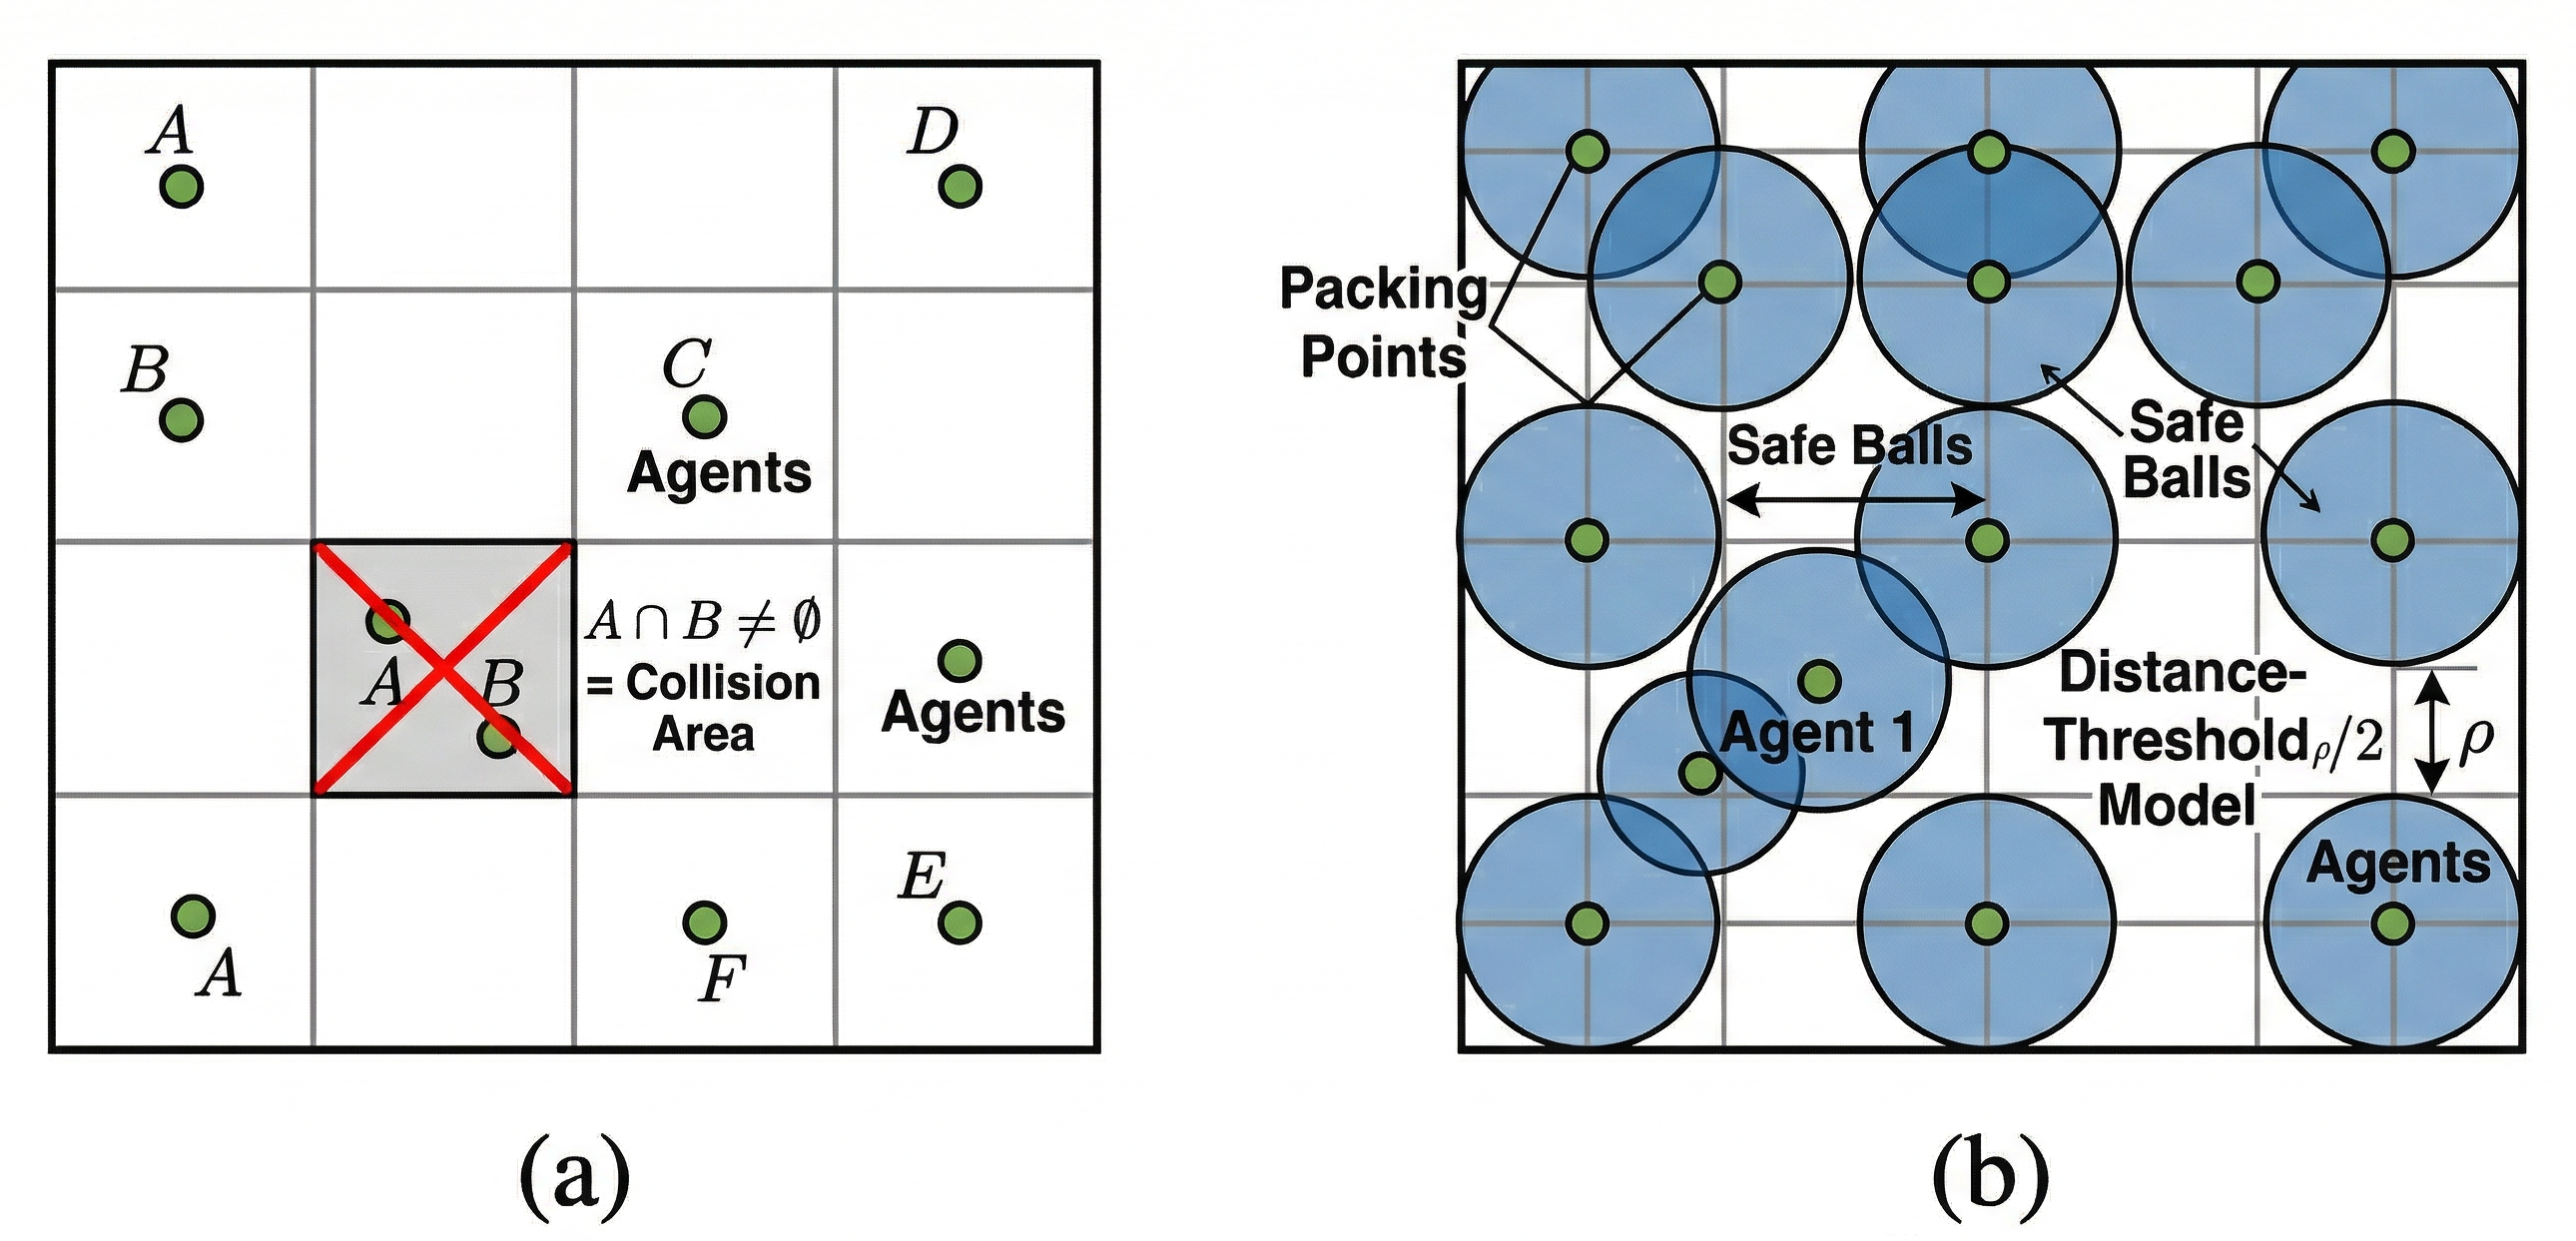
\includegraphics[width=0.45\textwidth]{img/packing-partition__1_.png}
  \caption{\textbf{Collision Geometries}. (a) The partition model discretizes the action space $\mathcal{X}$ into $K$ disjoint hypercubic cells; collisions occur when multiple players occupy the same cell. (b) The distance-threshold model manages interference by seating players within safe balls $B_i$ of radius $\sigma$ around $r$-packing centers $z_i$, ensuring an inter-agent separation $>\rho$.}
  \label{fig:geometry}
\end{figure}

While this partition model provides a clean and practical foundation, our algorithmic framework is sufficiently general to accommodate other geometries. In later sections, we will show how our approach extends to a distance-threshold model, where a collision occurs if any two players' actions are within a certain Euclidean distance $\rho$ of each other (see Figure \ref{fig:geometry}(b)). That model is more suited to applications like mobile robotics or sensor networks where interference is governed by physical proximity. By first solving the partition-based problem, we establish the core algorithmic principles in a clear and simple setting.

\subsection{Performance Benchmark and Objective}

The collision model imposes a fundamental constraint: at most one player can earn a non-zero reward from any given cell $C$ in a single round. It is therefore inappropriate to compare the system's performance to the ideal single-player benchmark of $N \cdot \sup_{x \in \X} \mu(x)$, as this might require all $N$ players to occupy the same infinitesimally small region. A principled comparator must respect this feasibility constraint.

We therefore define the benchmark based on the best possible static assignment of players to $N$ distinct cells. For each cell $C \in \Pcal$, let its optimal value be its cell-wise supremum, $\mu^\ast(C) := \sup_{x\in C}\mu(x)$. Let $\mu^\ast_{(1)}\ge \mu^\ast_{(2)}\ge\dots\ge \mu^\ast_{(K)}$ be these values sorted in nonincreasing order. The optimal collision-feasible reward in a single round is the sum of the top $N$ cell maxima: $\OPT_{\cont}(\Pcal,N) \;:=\; \sum_{m=1}^N \mu^\ast_{(m)}$.

The cumulative regret of a decentralized policy $\pi$ over a horizon $T$ is the difference between this optimal benchmark and the expected total reward collected by all players:

\begin{equation}
\label{eq:cont-regret}
\begin{aligned}
R_{\cont}(T; \pi, \Pcal, N) &:= T \cdot \OPT_{\cont}(\Pcal, N) \\
&\quad - \EE_\pi \! \left[ \sum_{t=1}^T \sum_{j=1}^N r_t^{(j)} \right],
\end{aligned}
\end{equation}
where $r_t^{(j)}$ is the realized reward for player $j$ at round $t$. Note that the benchmark depends on the partition $\Pcal$. This is an intentional feature of the model, not an artifact of the analysis; the partition defines the physical collision geometry of the environment.


A subtlety in this continuous setting is the difference between a cell's center value, $\mu(x_C)$, and its true maximum, $\mu^\ast(C)$. While the Lipschitz property guarantees they are close - $|\mu^\ast(C) - \mu(x_C)| \le Lh\sqrt{d}/2$ - their relative ordering across cells can be completely different. For instance, a cell with a modest center value might contain a sharp peak near its boundary, making it more valuable than a cell with a higher center value that is relatively flat. Any successful algorithm must therefore be designed to identify cells based on their maxima, not just their centers.

We use $[m]$ for the set $\{1,\dots,m\}$. All of our guarantees are high-probability statements that hold simultaneously for all players, cells, and time steps. We manage this by defining a total failure probability budget $\delta_{\textrm{sys}}\in(0,1/4)$ and allocating portions of it, such as $\delta_{\text{I}}$ and $\delta_{\text{II}}$, to different phases of the algorithm. This ensures the entire system behaves as expected with probability at least $1-\delta_{\textrm{sys}}$.

Since this is, to our knowledge, the first work to extend decentralized multi-player bandits to Lipschitz continuous domains with hard collisions, we focus on the cleanest foundational setting: decentralized play with zero-reward collisions and fixed public geometry. Extensions to richer models are left for future work.

\section{OUR APPROACH: A MULTI-PHASE DECENTRALIZED PROTOCOL}

Before going into technical details, we present a high-level overview of our strategy. The core idea is to decouple the multi-agent coordination problem from the single-agent continuous optimization problem. We achieve this with a four-phase protocol where the first three phases are dedicated to coordination and incur a total cost that is \emph{independent} of the time horizon $T$ up to logarithmic factors coming from the failure probability.

\begin{itemize}
    \item \textbf{PHASE I: COARSE IDENTIFICATION.} For a fixed duration $T_0$, all players explore the space by sampling cell centers uniformly at random. This process is intentionally chaotic and communication-free. While many samples will result in collisions, we show that with high probability, every player obtains a sufficient number of successful, non-colliding observations from every cell to construct coarse but statistically valid confidence bounds on each cell's maximum value. The purpose of this phase is not to be precise, but to safely prune the vast majority of suboptimal cells.

    \item \textbf{PHASE II: USING MAXIMA FOR REFINEMENT.} Using the candidate cells identified in Phase I, players perform a localized ``peek" inside each one. They sample from a fine grid of points within each candidate cell to build high-resolution confidence bounds that tightly bracket the true cell maximum $\mu^\ast(C)$. This critical step corrects for the center-versus-maximum bias and allows us to identify the top-$N$ cells, even without a gap between the best and the rest.

    \item \textbf{PHASE II$\tfrac{1}{2}$: DECENTRALIZED SEATING.} Having agreed upon a common set of $N$ target cells, players must assign themselves to these cells without conflict. They use the Musical Chairs protocol, where unseated players repeatedly sample from the target set until they land on a free cell. We analyze the practical version of this protocol and show that all players are seated in expected $O(N)$ time.

    \item \textbf{PHASE III: WITHIN-CELL OPTIMIZATION.} Once each player is uniquely assigned to a high-quality cell, the multi-agent problem factorizes. For the remainder of the horizon, each player independently runs a single-player Lipschitz bandit algorithm confined to their assigned cell, efficiently optimizing their local reward.
\end{itemize}
This modular structure allows us to isolate and solve the challenges of coordination and learning sequentially, leading to a cleaner analysis. 


